\documentclass[11pt]{article}
\usepackage[margin=0.7in]{geometry}
\usepackage{amsmath,amssymb}
\usepackage{graphicx}
\usepackage{float}
\usepackage{xcolor}
\usepackage{listings}
\setlength{\parindent}{0pt}
\setlength{\parskip}{0.5em}
\lstset{
    language=Python,
    basicstyle=\ttfamily\footnotesize,
    keywordstyle=\color{blue},
    commentstyle=\color{green!50!black},
    stringstyle=\color{red!50!black},
    numbers=left,
    numberstyle=\tiny\color{gray},
    frame=single,
    breaklines=true
}

\begin{document}

\section*{2.1 Cart-Pole Swing-Up with Limited Actuation}

\subsection*{2.1(a)}
At SCP iteration \(i\), linearize \(f_d\) around
\((s_k^{(i)},u_k^{(i)})\):
\[
    s_{k+1}=A_k s_k+B_k u_k+c_k,
\]
where
\[
    A_k=\frac{\partial f_d}{\partial s}(s_k^{(i)},u_k^{(i)}),\qquad
    B_k=\frac{\partial f_d}{\partial u}(s_k^{(i)},u_k^{(i)}),
\]
\[
    c_k=f_d(s_k^{(i)},u_k^{(i)})-A_k s_k^{(i)}-B_k u_k^{(i)}.
\]
The convex subproblem is
\[
\begin{aligned}
\min_{s,u}\quad
&\sum_{k=0}^{N-1}\left((s_k-s_{\rm goal})^TQ(s_k-s_{\rm goal})+u_k^TRu_k\right)
 +(s_N-s_{\rm goal})^TP(s_N-s_{\rm goal})\\
\text{s.t.}\quad
&s_0=\bar s_0,\\
&s_{k+1}=A_k s_k+B_k u_k+c_k,\\
&-u_{\max}\le u_k\le u_{\max},\\
&\|s_k-s_k^{(i)}\|_\infty\le \rho,\qquad
  \|u_k-u_k^{(i)}\|_\infty\le \rho.
\end{aligned}
\]

\subsection*{2.1(b)}
The requested JAX implementation is:
\begin{lstlisting}
A, B = jax.jacobian(fd, argnums=(0, 1))(sbar, ubar)
c = fd(sbar, ubar) - A @ sbar - B @ ubar
\end{lstlisting}

\subsection*{2.1(c)}
The implementation is in \texttt{code/cartpole\_swingup\_constrained.py}. The
function \texttt{scp\_iteration} creates CVXPY variables for \(s\) and \(u\),
adds the linearized dynamics, box input constraints, trust region constraints,
and minimizes the convex quadratic cost above.

\subsection*{2.1(d)}
To swing up and then keep the pendulum upright, first use SCP to compute a
feasible swing-up trajectory. Once the pendulum is near
\((0,\pi,0,0)\), switch to a local LQR stabilizing controller designed around
the upright equilibrium. This gives a hybrid controller: SCP for the large
nonlinear maneuver, then LQR for local stabilization.

\begin{figure}[H]
\centering
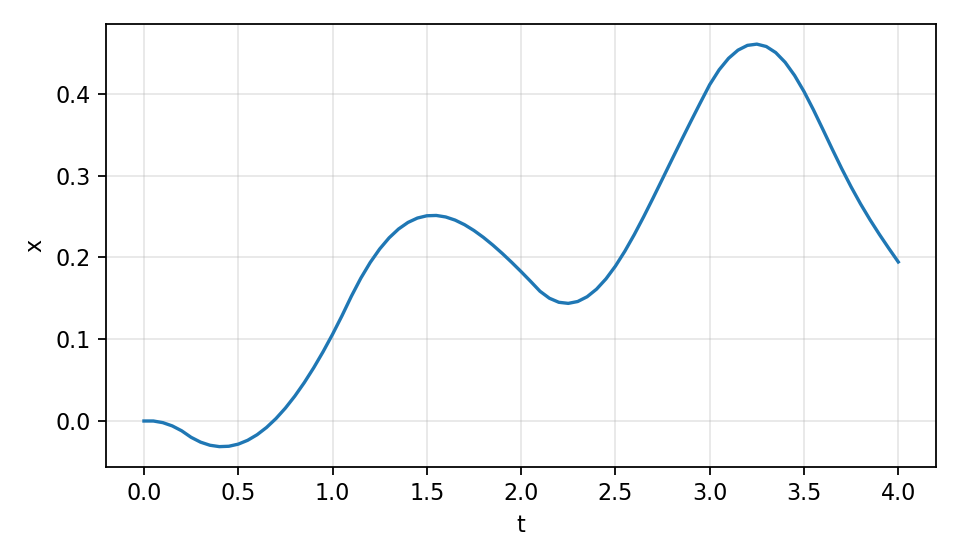
\includegraphics[width=0.45\textwidth]{figures/p21_state_x.png}
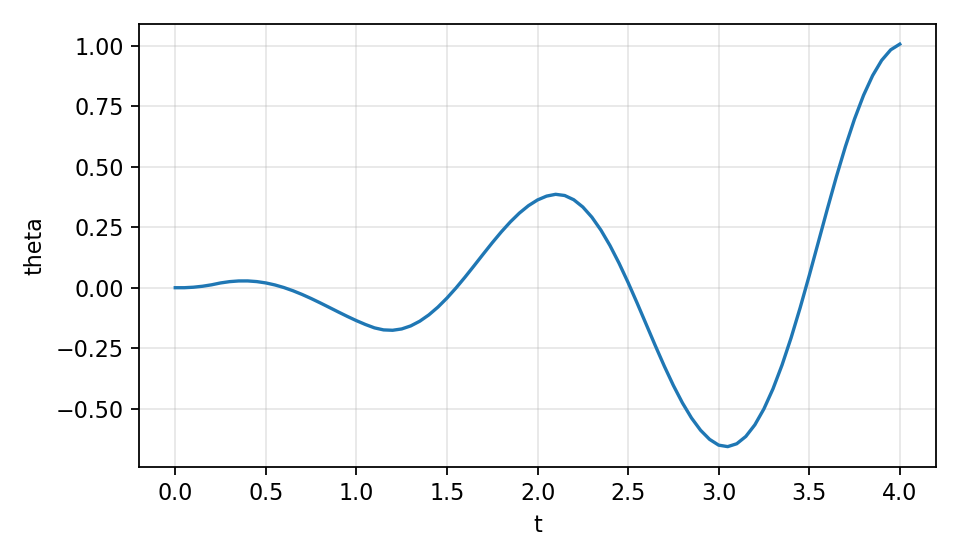
\includegraphics[width=0.45\textwidth]{figures/p21_state_theta.png}
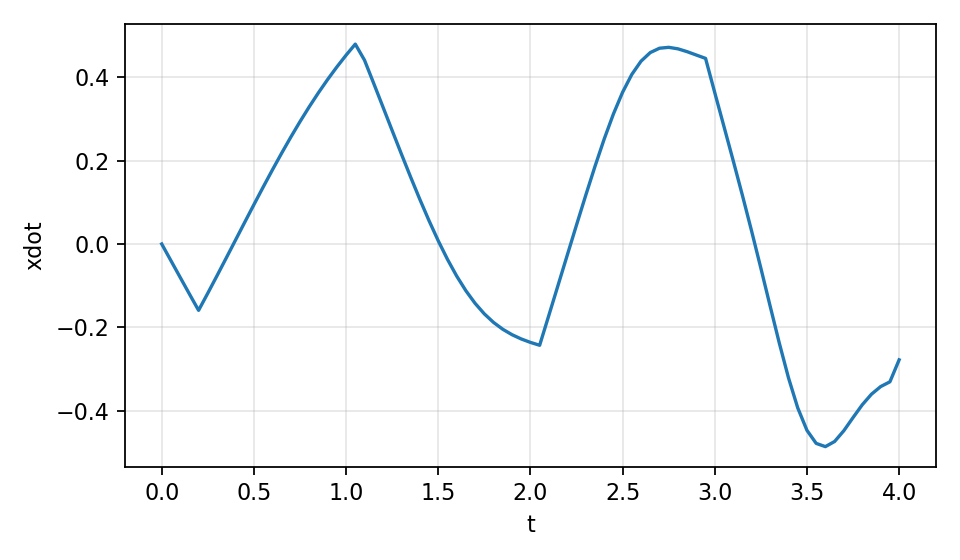
\includegraphics[width=0.45\textwidth]{figures/p21_state_xdot.png}
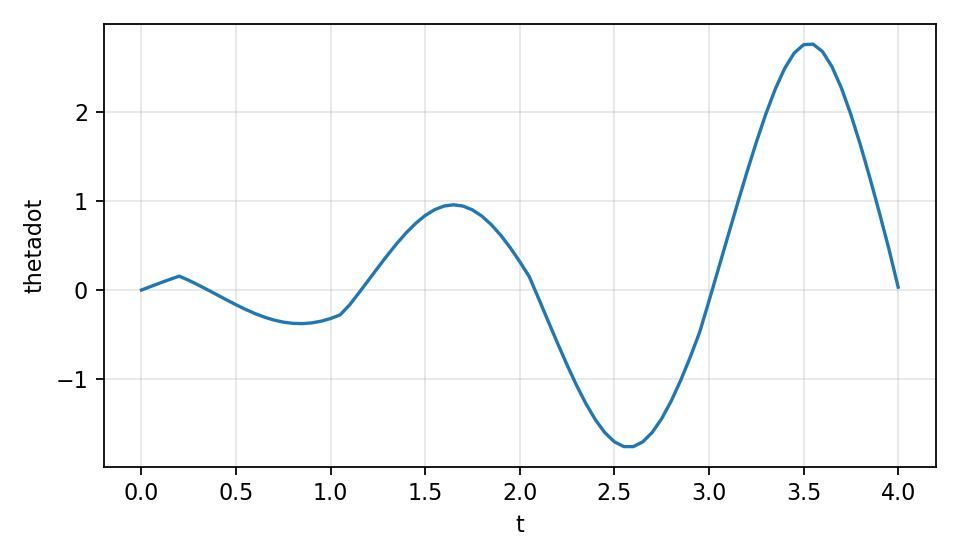
\includegraphics[width=0.45\textwidth]{figures/p21_state_thetadot.png}
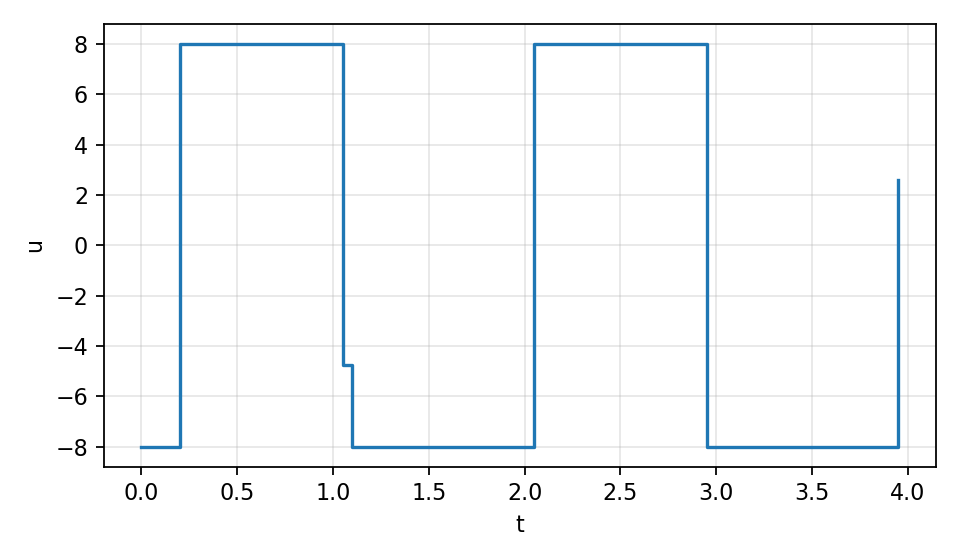
\includegraphics[width=0.45\textwidth]{figures/p21_control.png}
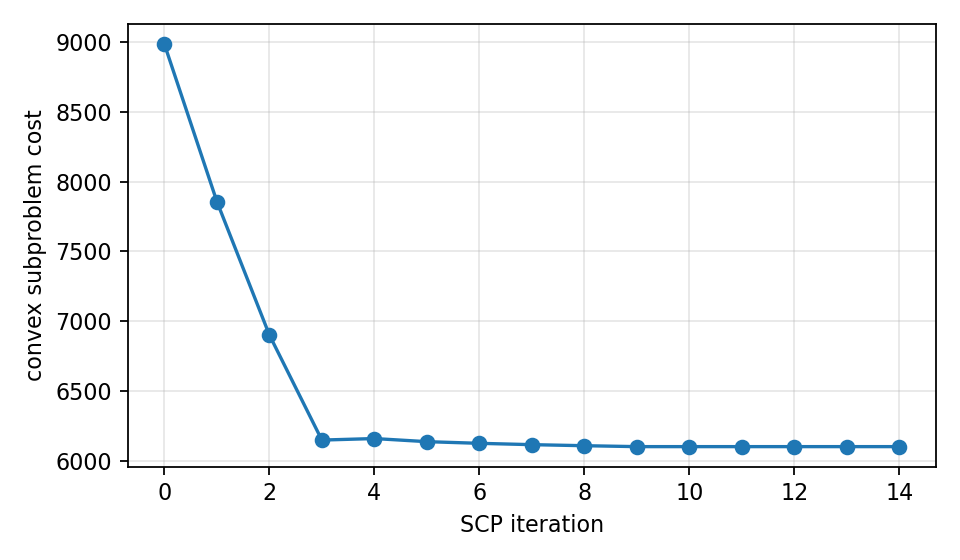
\includegraphics[width=0.45\textwidth]{figures/p21_scp_cost.png}
\caption{SCP swing-up trajectory with bounded input and trust-region updates.}
\end{figure}

\section*{2.2 Shortest Path Through a Grid}

\subsection*{2.2(a)}
Using dynamic programming from right to left gives the value function
\[
\begin{array}{c|c}
\text{node} & V(\text{node})\\
\hline
B&0\\
u_5&10\\
d_5&11\\
u_4&18\\
m_4&16\\
d_4&20\\
u_3&25\\
um_3&23\\
dm_3&21\\
d_3&27\\
u_2&29\\
m_2&29\\
d_2&31\\
u_1&35\\
d_1&36\\
A&40
\end{array}
\]
Thus the shortest path has cost
\[
    \boxed{40}.
\]
One optimal path is
\[
    A\to u_1\to u_2\to um_3\to u_4\to u_5\to B.
\]

\subsection*{2.2(b)}
For an \(n\)-segment grid, each route consists of \(n\) up moves and \(n\) down
moves, so exhaustive search evaluates
\[
    \boxed{\binom{2n}{n}}
\]
routes. Dynamic programming evaluates each nonterminal node. The number of
such DP evaluations is
\[
    \boxed{n(n+2)}.
\]
For \(n=3\), these give \(\binom{6}{3}=20\) and \(3(5)=15\), matching the
problem statement.

\section*{2.3 Cart-Pole Balance}

\subsection*{2.3(a)}
With \(\tilde s_k=s_k-\bar s\), Euler discretization gives
\[
    \tilde s_{k+1}\approx A\tilde s_k+Bu_k,
\]
where
\[
    A=I+\Delta t
    \begin{bmatrix}
    0&0&1&0\\
    0&0&0&1\\
    0&\frac{m_pg}{m_c}&0&0\\
    0&\frac{(m_c+m_p)g}{m_c\ell}&0&0
    \end{bmatrix},
    \qquad
    B=\Delta t
    \begin{bmatrix}
    0\\0\\ \frac{1}{m_c}\\ \frac{1}{m_c\ell}
    \end{bmatrix}.
\]

\subsection*{2.3(b)}
Using Riccati recursion until
\(\|P_k-P_{k-1}\|_{\max}<10^{-4}\) gives
\[
    \boxed{K_\infty=
    \begin{bmatrix}
    0.73&-231.85&4.22&-68.25
    \end{bmatrix}.}
\]

\subsection*{2.3(c)}
\begin{figure}[H]
\centering
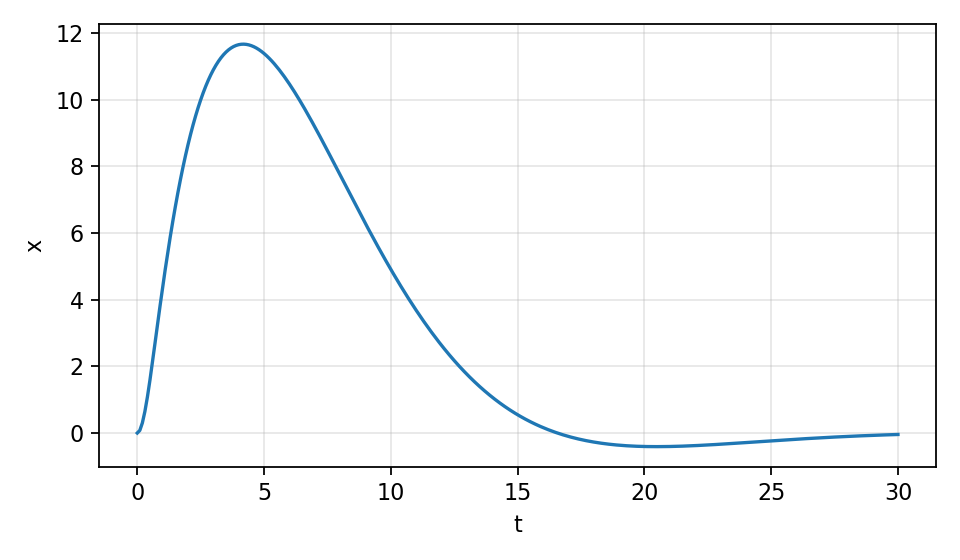
\includegraphics[width=0.45\textwidth]{figures/p23_balance_x.png}
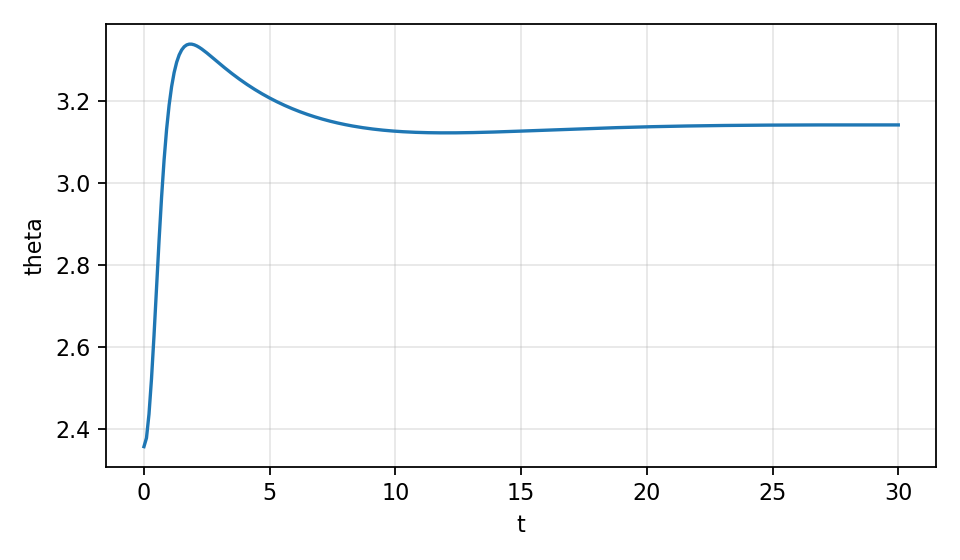
\includegraphics[width=0.45\textwidth]{figures/p23_balance_theta.png}
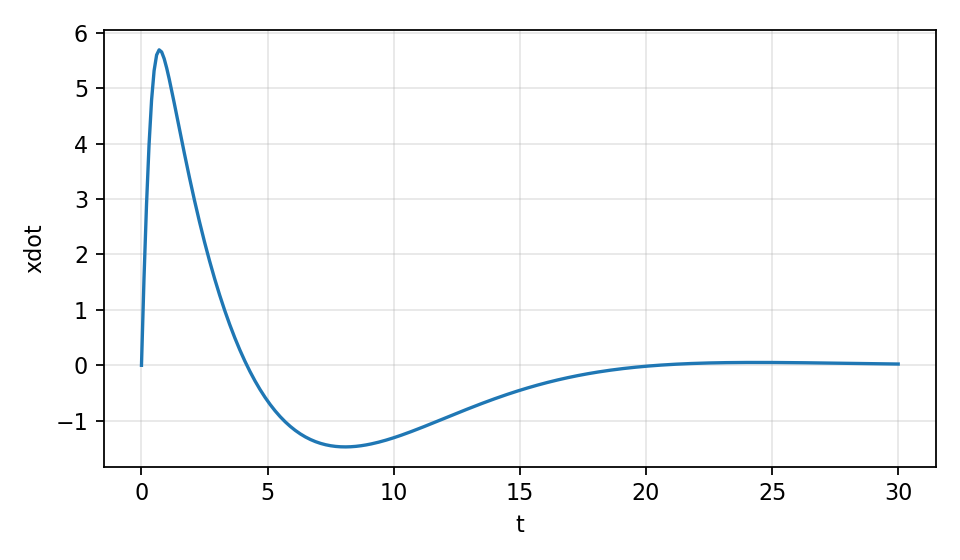
\includegraphics[width=0.45\textwidth]{figures/p23_balance_xdot.png}
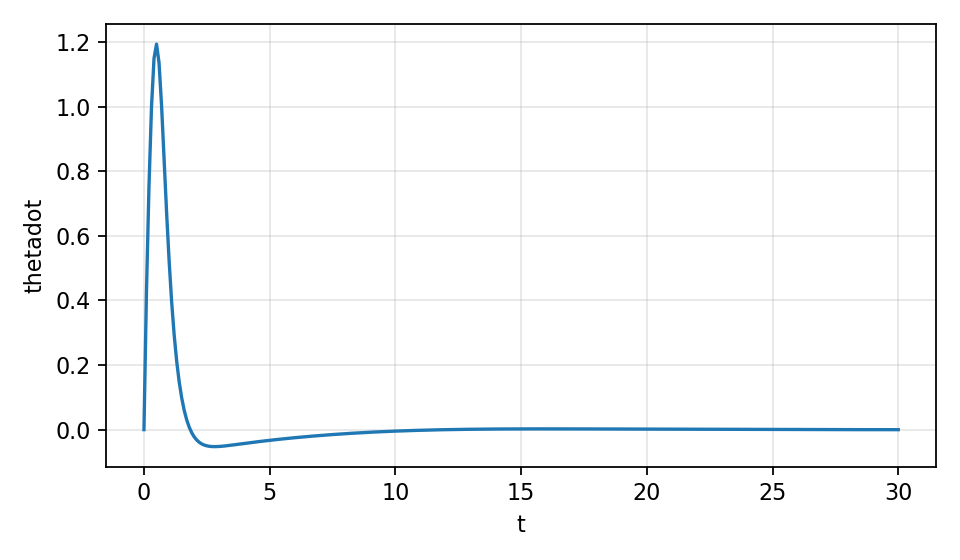
\includegraphics[width=0.45\textwidth]{figures/p23_balance_thetadot.png}
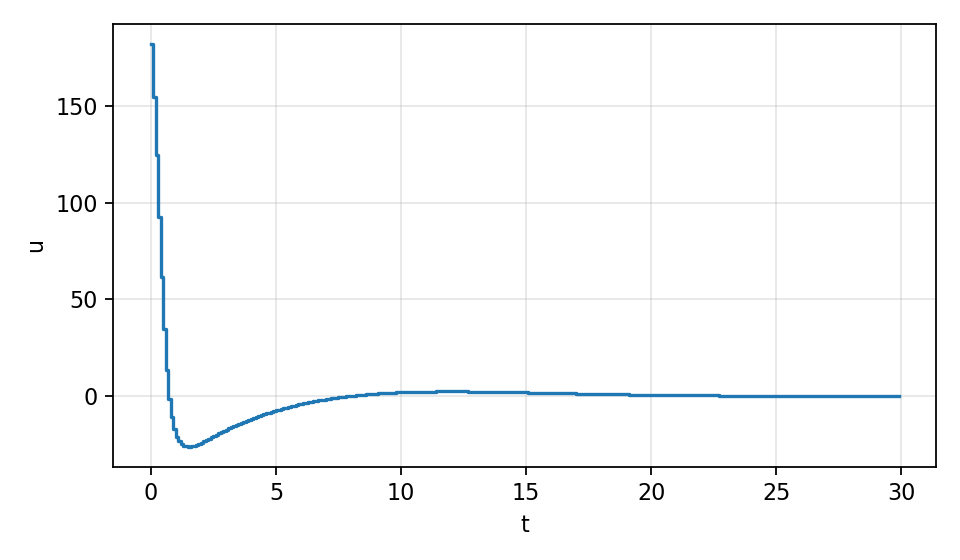
\includegraphics[width=0.45\textwidth]{figures/p23_balance_u.png}
\caption{Cart-pole balance with the infinite-horizon LQR controller.}
\end{figure}

\subsection*{2.3(d)}
\textbf{i.} We can reuse \(A\) and \(B\) because the dynamics Jacobians along
the reference do not depend on \(x\), and the desired trajectory keeps
\(\theta=\pi\), \(\dot\theta=0\). Therefore the same upright linearization is
valid along the reference.

\textbf{ii.}
\begin{figure}[H]
\centering
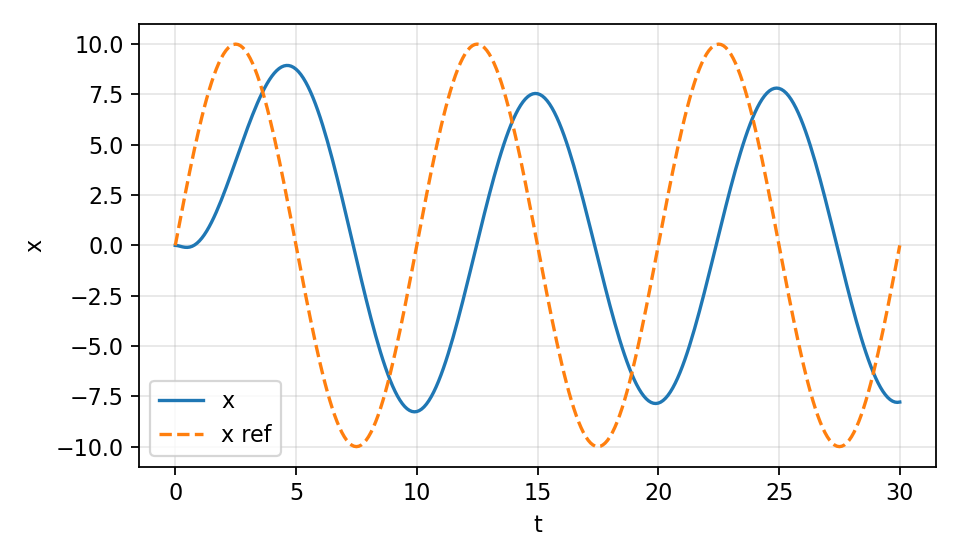
\includegraphics[width=0.45\textwidth]{figures/p23_tracking_x.png}
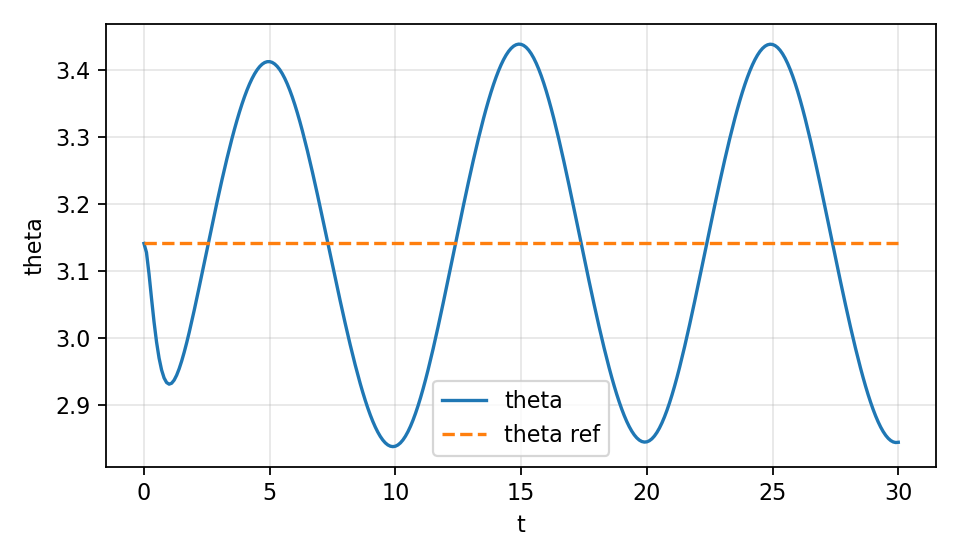
\includegraphics[width=0.45\textwidth]{figures/p23_tracking_theta.png}
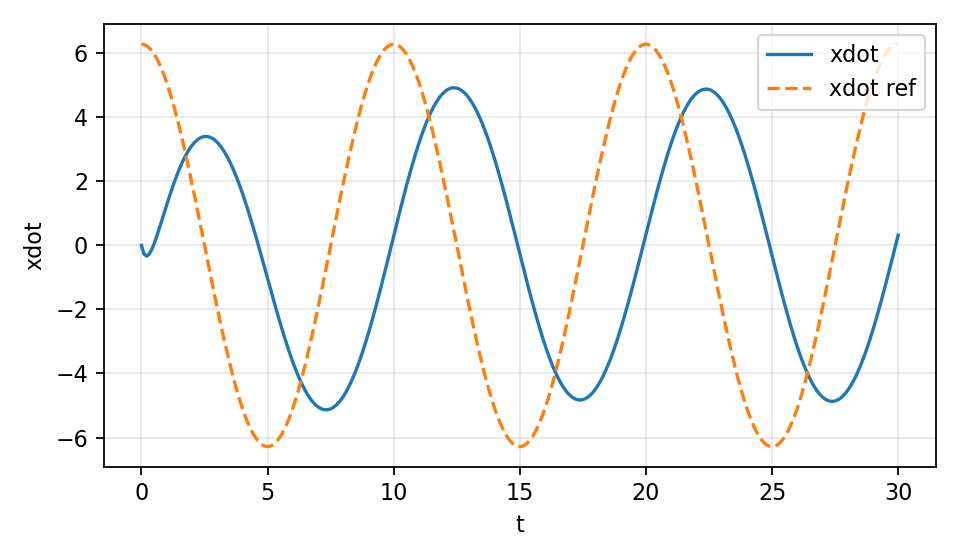
\includegraphics[width=0.45\textwidth]{figures/p23_tracking_xdot.png}
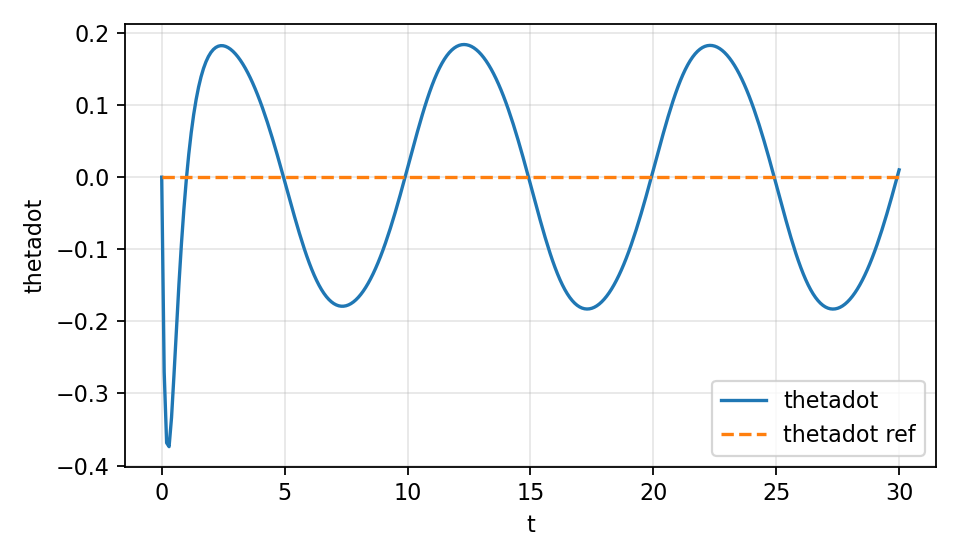
\includegraphics[width=0.45\textwidth]{figures/p23_tracking_thetadot.png}
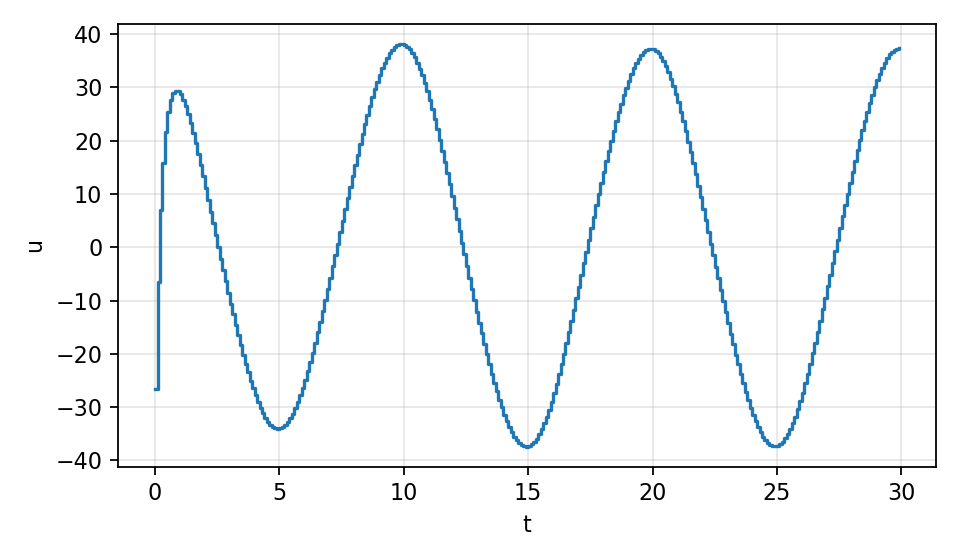
\includegraphics[width=0.45\textwidth]{figures/p23_tracking_u.png}
\caption{Tracking \(x_{\rm ref}(t)=10\sin(2\pi t/10)\) with LQR feedback.}
\end{figure}

\textbf{iii.} The reference cart motion has nonzero acceleration, but the
reference does not include a dynamically consistent feedforward force. The
pendulum must tilt to generate the horizontal cart acceleration, so keeping
\(\theta(t)\equiv\pi\) while moving the cart sinusoidally is not a dynamically
consistent upright trajectory without feedforward compensation.

\section*{2.4 Cart-Pole Swing-Up}

\subsection*{2.4(a)}
The requested one-line JAX linearization is
\begin{lstlisting}
A, B = jax.jacobian(fd, argnums=(0, 1))(sbar_k, ubar_k)
\end{lstlisting}

\subsection*{2.4(b)}
Let
\[
    \tilde s_k=s_k-\bar s_k,\qquad \tilde u_k=u_k-\bar u_k.
\]
Expanding the quadratic cost gives linear terms
\[
    q_N=Q_N(\bar s_N-s_{\rm goal}),\qquad
    q_k=Q(\bar s_k-s_{\rm goal}),\qquad
    r_k=R\bar u_k.
\]

\subsection*{2.4(c)}
The iLQR implementation is in \texttt{code/cartpole\_swingup.py}. It computes
linearizations, performs the Riccati backward pass for feedback gains \(Y_k\)
and offsets \(y_k\), updates the nominal trajectory, and uses backtracking to
keep the update stable.

\subsection*{2.4(d)}
\begin{figure}[H]
\centering
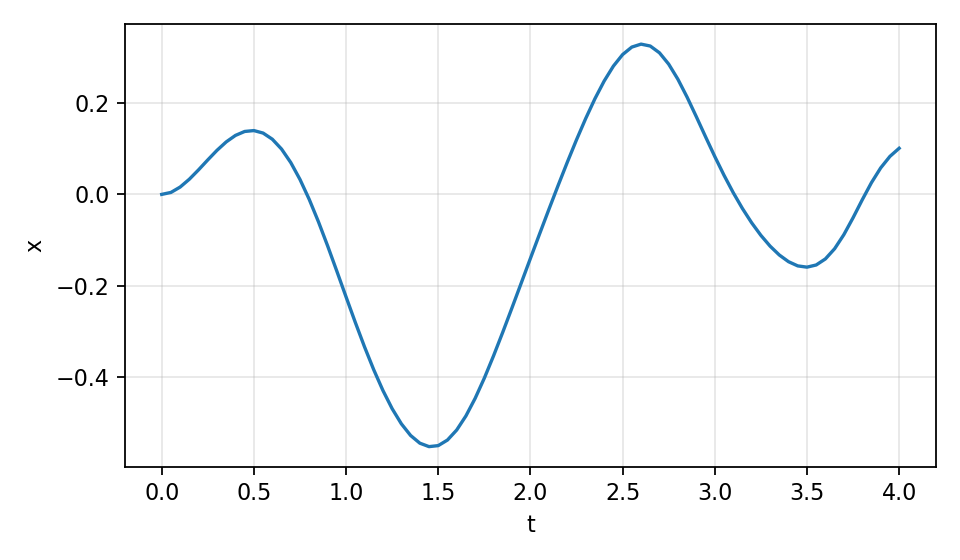
\includegraphics[width=0.45\textwidth]{figures/p24_open_loop_x.png}
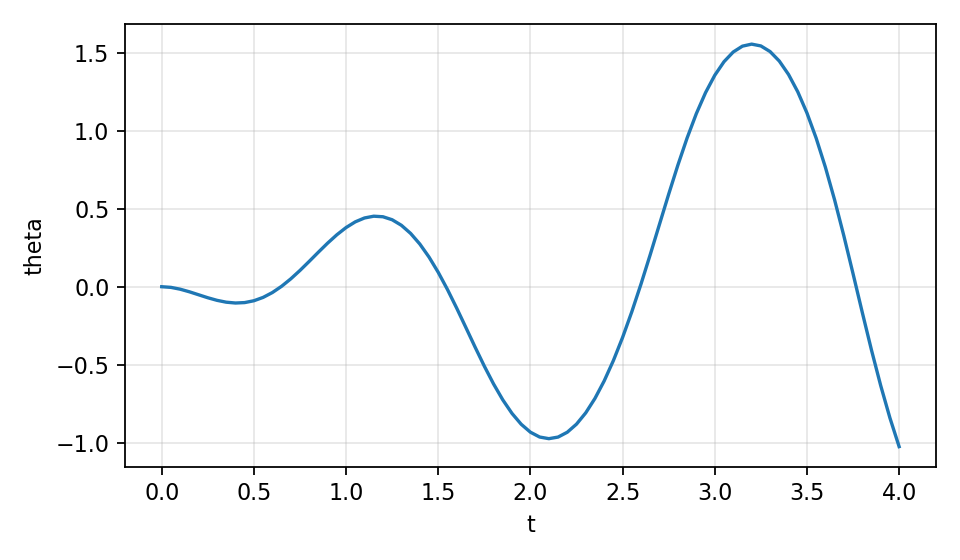
\includegraphics[width=0.45\textwidth]{figures/p24_open_loop_theta.png}
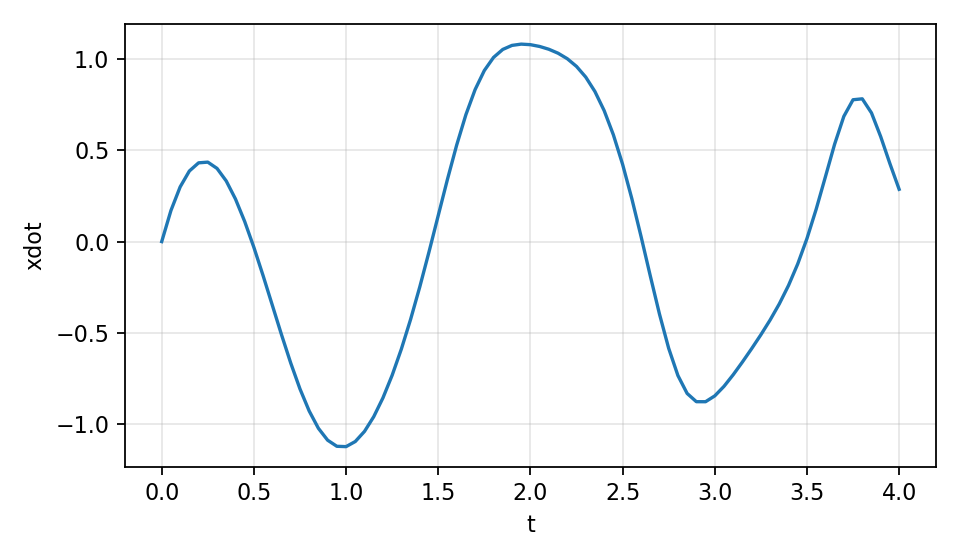
\includegraphics[width=0.45\textwidth]{figures/p24_open_loop_xdot.png}
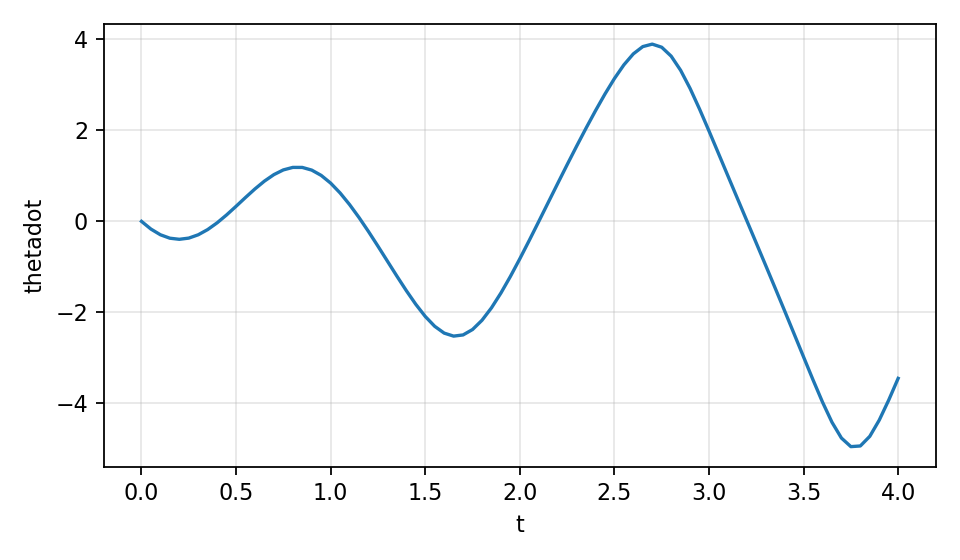
\includegraphics[width=0.45\textwidth]{figures/p24_open_loop_thetadot.png}
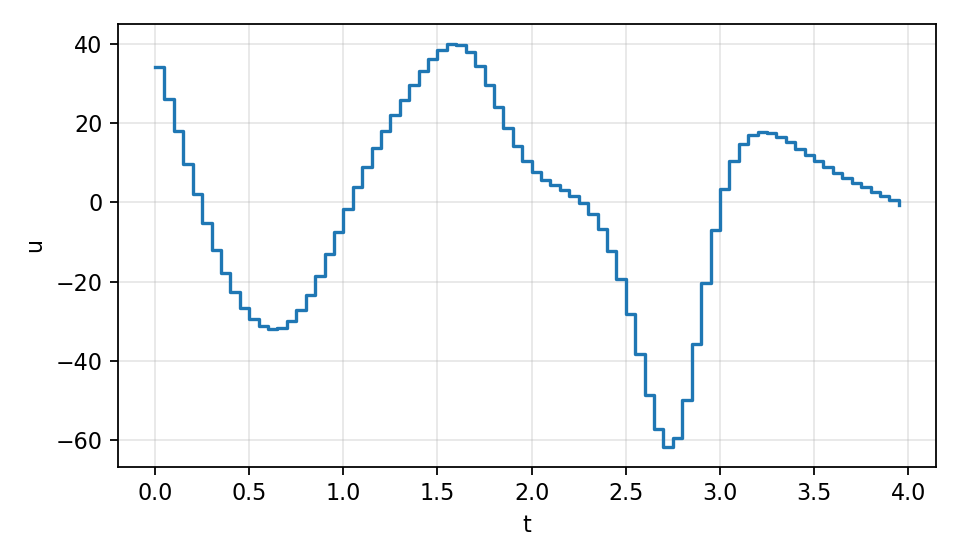
\includegraphics[width=0.45\textwidth]{figures/p24_open_loop_u.png}
\caption{Open-loop application of the iLQR control sequence.}
\end{figure}

\begin{figure}[H]
\centering
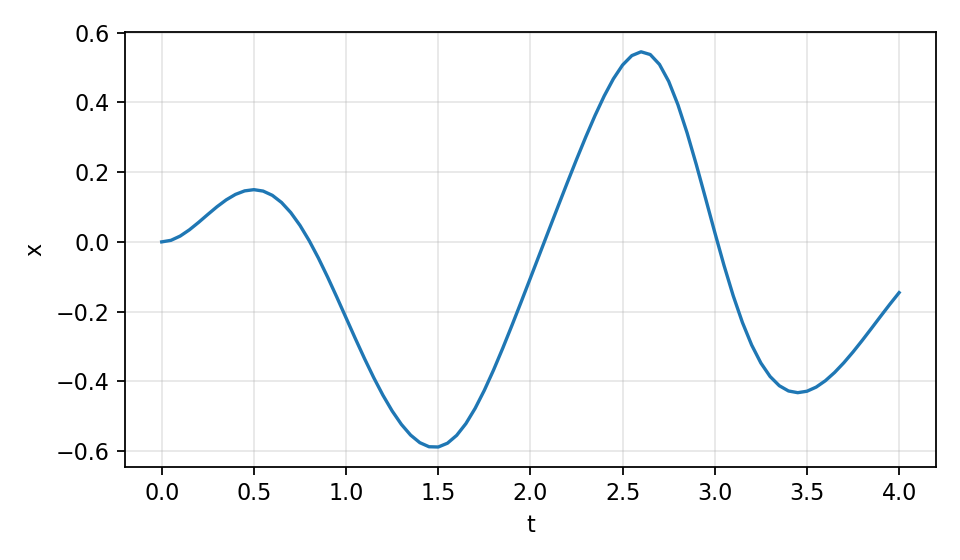
\includegraphics[width=0.45\textwidth]{figures/p24_closed_loop_x.png}
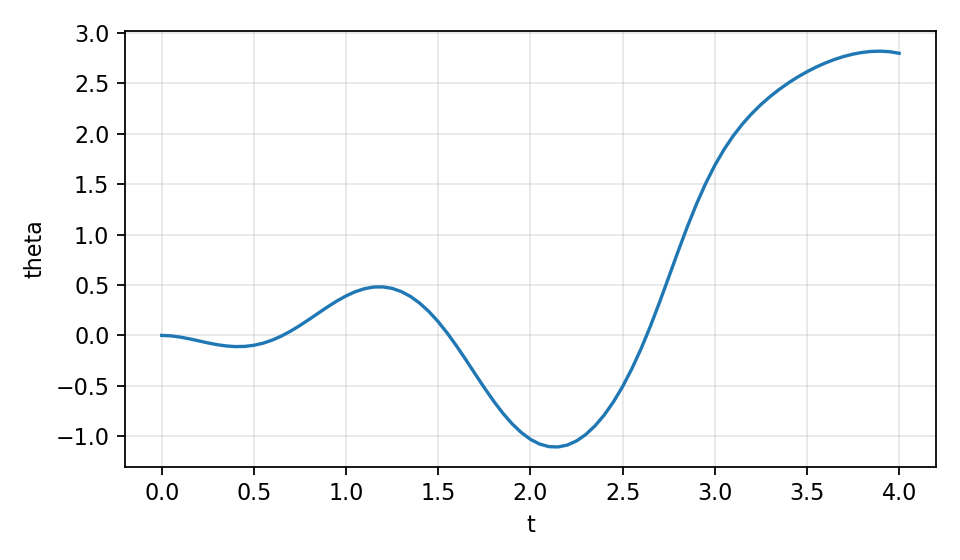
\includegraphics[width=0.45\textwidth]{figures/p24_closed_loop_theta.png}
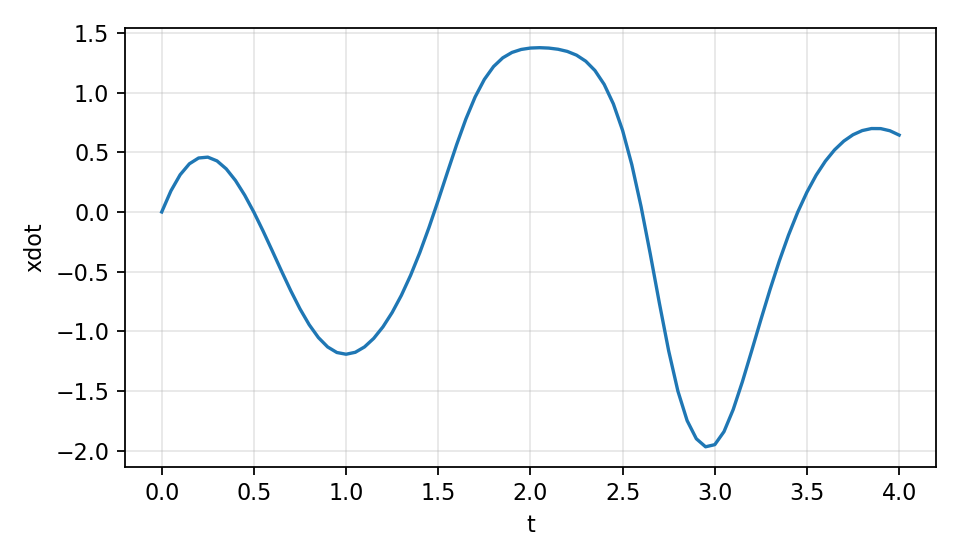
\includegraphics[width=0.45\textwidth]{figures/p24_closed_loop_xdot.png}
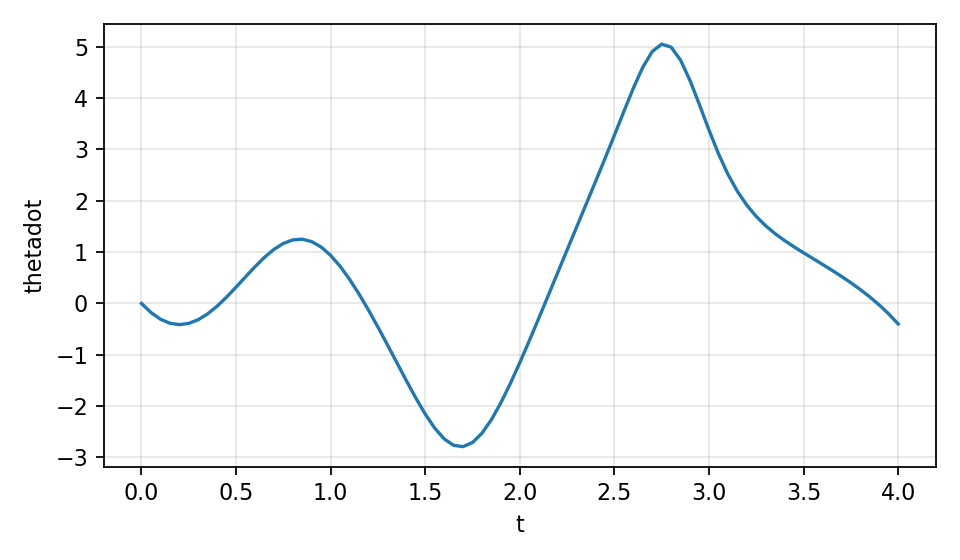
\includegraphics[width=0.45\textwidth]{figures/p24_closed_loop_thetadot.png}
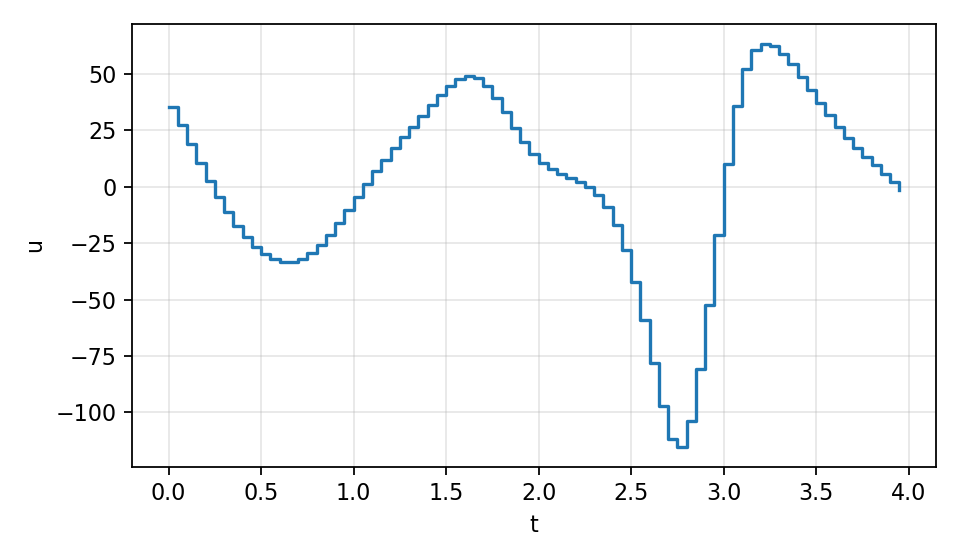
\includegraphics[width=0.45\textwidth]{figures/p24_closed_loop_u.png}
\caption{Closed-loop iLQR policy.}
\end{figure}

\section*{2.5 Machine Maintenance}

Let \(V_R(h)\) and \(V_B(h)\) denote the optimal expected profit with \(h\)
weeks remaining when the machine starts the week running or broken.
\[
\begin{aligned}
V_R(h)&=\max\{40+0.6V_R(h-1)+0.4V_B(h-1),\\
&\qquad\qquad 30+0.3V_R(h-1)+0.7V_B(h-1)\},\\
V_B(h)&=\max\{20+0.6V_R(h-1)+0.4V_B(h-1),\ -50+V_R(h-1)\}.
\end{aligned}
\]
With \(V_R(0)=V_B(0)=0\), the computed values are
\[
\begin{array}{c|cccc}
h&0&1&2&3\\
\hline
V_R(h)&0&40&72&104\\
V_B(h)&0&20&52&84
\end{array}
\]
The optimal policy is to perform preventive maintenance when running and to
repair when broken. Since the machine is new at week 1 and guaranteed to run
through that week, the total expected profit over four weeks is
\[
    \boxed{100+V_R(3)=204}.
\]

\end{document}
